\section*{Exercises for Section~\ref{S:mathinduction}}
%
\begin{enumerate}

\xitem Which of the following sets are inductive sets?  Explain. \label{exer:sec51-1}
\begin{multicols}{2}
\begin{enumerate}
  \item $\mathbb{Z}$
  \item $\left\{ {x \in \mathbb{N} \mid x \geq 4} \right\}$
  \item $\left\{ {x \in \mathbb{Z} \mid x \leq 10} \right\}$
  \item $\left\{ {1,2,3, \ldots ,500} \right\}$
\end{enumerate}
\end{multicols}

\xitem \label{exer:sec51-2} \begin{enumerate} 
  \item Can a finite, nonempty set be inductive?  Explain.
  \item Is the empty set inductive?  Explain.
\end{enumerate}

%\item Let $P \left( n \right)$   be the predicate \label{exer:indstep}
%$1 + 2 +  \cdots  + n = \dfrac{{n^2  + n + 1}}{2}$.
%\begin{enumerate}
%  \item Let  $k \in \mathbb{N}$.  Complete the following proof that if  $P\left( k \right)$ is true, then  $P\left( {k + 1} \right)$ is true.  If $P \left( k \right)$ is ture, then
%%
%\[
%1 + 2 +  \cdots  + k = \frac{{k^2  + k + 1}}{2}.
%\]
%%
%The goal is to prove that  $P\left( {k + 1} \right)$ is true.  That is, we need to prove that
%%
%\[
%1 + 2 +  \cdots  + k + \left( {k + 1} \right) = \frac{{\left( {k + 1} \right)^2  + \left( {k + 1} \right) + 1}}{2}.
%\]
%
%To do this, we add  $\left( {k + 1} \right)$ to both sides of Equation~(\ref{eq:act16a}).  This gives \ldots
%\[
%\begin{aligned}
%  1 + 2 +  \cdots  + k + \left( {k + 1} \right) &= \frac{{k^2  + k + 1}}{2} + \left( {k + 1} \right) \\ 
%                                                &=  \cdots.  \\ 
%\end{aligned}
%\]

%  \item Is  $P\left( 1 \right)$ true?  Is  $P\left( 2 \right)$ true?  What about $P\left( 3 \right)$ and $P\left( 4 \right)$?  Explain how this shows that the basis step is an essential part of a proof by induction.
%\end{enumerate}


\item Use mathematical induction to prove each of the following: \label{exer:sec51-3}

\begin{enumerate}
%  \item For each natural number  $n$,  $1 + 2 + 3 +  \cdots  + n = \dfrac{{n\left( {n + 1} \right)}}{2}$.  
%Or, using summation notation, for each natural number  $n$,  
%\[
%\sum\limits_{j = 1}^n j  = \dfrac{{n\left( {n + 1} \right)}}{2}.
%\] \label{exer:51-3a}

\yitem For each natural number  $n$,  
$2 + 5 + 8 +  \cdots  + \left( {3n - 1} \right) = \dfrac{{n\left( {3n + 1} \right)}}{2}$. 
\label{exer:inductionsum-a} 
%Or, using summation notation, for each natural number  $n$, 
%\[
%\sum\limits_{j = 1}^n {\left( {3j - 1} \right)}  = \dfrac{{n\left( {3n + 1} \right)}}{2}.
%\]
\item For each natural number $n$, 
$1 + 5 + 9 + \cdots + \left(4n - 3 \right) = n \left(2n - 1 \right)$.

\item For each natural number  $n$, 
$1^3 + 2^3 + 3^3 + \cdots + n^3 =  \left[ {\dfrac{{n\left( {n + 1} \right)}}{2}} \right]^2$.
\label{exer:51-3c}
%\[ 
%\sum\limits_{j = 1}^n {j^3 }  = \left[ {\dfrac{{n\left( {n + 1} \right)}}{2}} \right]^2. 
%\] 
\end{enumerate}

\item  Based on the results in Progress Check~\ref{prog:indexample} and 
Exercise~(\ref{exer:51-3c}), if  $n \in \mathbb{N}$, is there any conclusion that can be made about the relationship between the sum $\left( {1^3  + 2^3  + 3^3  +  \cdots  + n^3 } \right)$
 and the sum $\left( {1 + 2 + 3 +  \cdots  + n} \right)$?
 

\item Instead of using induction, we can sometimes use previously proven results about a summation to obtain results about a different summation. \label{exer:previnduction}
\begin{enumerate} 
\item Use the result in Progress Check~\ref{prog:indexample} to prove the following proposition:
\begin{center}
For each natural number  $n$,  $3 + 6 + 9 +  \cdots  + 3n = \dfrac{{3n\left( {n + 1} \right)}}{2}$.
\end{center}
\label{exer:previnduction-a}

\item Subtract $n$ from each side of the equation in Part~(a).  On the left side of this equation, explain why this can be done by subtracting $1$ from each term in the summation. \label{exer:previnduction-b}

\item Algebraically simplify the right side of the equation in Part~(b) to obtain a formula for the sum $2 + 5 + 8 + \cdots + \left( 3n - 1 \right)$.  Compare this to 
Exercise~(\ref{exer:inductionsum-a}).
\end{enumerate}

\xitem \label{exer:sec51-5} \begin{enumerate} \item Calculate  
$1 + 3 + 5 +  \cdots  + \left( {2n - 1} \right)$
for several natural numbers  $n$. \label{exer:515a}

\item Based on your work in Exercise~(\ref{exer:515a}), if  $n \in \mathbb{N}$, make a conjecture about the value of  the sum $1 + 3 + 5 +  \cdots  + \left( {2n - 1} \right) = \sum\limits_{j = 1}^n {\left( {2j - 1} \right)} $.  \label{exer:515b}

\item Use mathematical induction to prove your conjecture in Exercise~(\ref{exer:515b}).
\end{enumerate}

\item In Section~\ref{S:directproof}, we defined congruence modulo  $n$  for a natural number 
$n$, and in Section~\ref{S:divalgo}, we used the Division Algorithm to prove that each integer is congruent, modulo  $n$, to precisely one of the integers  $0,1,2, \ldots ,n - 1$ (Corollary~\ref{C:congtorem}). \label{exer:mod3conjecture}

\begin{enumerate}
\item Find the value of  $r$  so that   $4 \equiv r \pmod 3$ and  $r \in \left\{ {0,1,2} \right\}$.

\item Find the value of  $r$  so that   $4^2  \equiv r \pmod 3$ and  $r \in \left\{ {0,1,2} \right\}$.

\item Find the value of  $r$  so that   $4^3  \equiv r \pmod 3$  and  $r \in \left\{ {0,1,2} \right\}$.

\item For two other values of $n$, find the value of  $r$  so that   $4^n  \equiv r \pmod 3$  and  $r \in \left\{ {0,1,2} \right\}$.

\yitem If  $n \in \mathbb{N}$, make a conjecture concerning the value of  $r$  where  \\
$4^n  \equiv r \pmod 3$  and  $r \in \left\{ {0,1,2} \right\}$.  This conjecture should be written as a self-contained proposition including an appropriate quantifier.

\yitem Use mathematical induction to prove your conjecture.

\end{enumerate}




\item Use mathematical induction to prove each of the following: \label{exer:sec51-6}
\begin{enumerate}
  \yitem For each natural number  $n$,  3 divides $\left( {4^n  - 1} \right)$. \label{exer:516a}

  \item For each natural number  $n$,  6 divides $\left( {n^3  - n} \right)$.
\end{enumerate}


\item In Exercise~(\ref{exer:mod3conjecture}), we proved that for each natural number  $n$,  
$4^n  \equiv 1 \pmod 3$.    Explain how this result is related to the proposition in Exercise~(\ref{exer:516a}).


\item Use mathematical induction to prove that for each natural number $n$, 3 divides 
$n^3 + 23n$.  Compare this proof to the proof from Exercise~(\ref{exer:case-ind}) in Section~\ref{S:divalgo}.


\item \label{exer:sec51-8}
\begin{enumerate} 
\item Calculate the value of $5^n - 2^n$ for $n = 1$, $n = 2$, $n = 3$, $n = 4$, $n = 5$, and 
$n = 6$. \label{exer:sec51-8a}
%\item Complete the following table: \label{exer:sec51-8a}
%
%\begin{center}
%\begin{tabular}{|c | c | c | c | c |} \cline{1-2} \cline{4-5}
%  $n$  &  $\left( {5^n  - 2^n } \right)$  &  &  $n$  &  $\left( {5^n  - 2^n } \right)$ \\ \cline{1-2} \cline{4-5}
%  $1$  &    &      &   $5$    &        \\ \cline{1-2} \cline{4-5}
%  $2$  &    &      &   $6$    &        \\ \cline{1-2} \cline{4-5}
%  $3$  &    &      &   $7$    &        \\ \cline{1-2} \cline{4-5}
%  $4$  &    &      &   $8$    &        \\ \cline{1-2} \cline{4-5}
%\end{tabular}
%\end{center}

  \item Based on your work in Part~(a), make a conjecture about the values of  $5^n  - 2^n $ for each natural number  $n$.  \label{exer:sec51-8b}
  \item Use mathematical induction to prove your conjecture in Part~(b).
\end{enumerate}

\item Let $x$ and $y$ be distinct integers.  Prove that for each natural number $n$, $\left( x - y \right)$ divides $\left( x^n - y^n \right)$.  Explain why your conjecture in 
Exercise~(\ref{exer:sec51-8}) is a special case of this result.

\xitem Prove Part~(\ref{T:propsofcong3}) of Theorem~\ref{T:propsofcong} from Section~\ref{S:cases}.
Let  $n \in \mathbb{N}$ and let  $a$ and $b$ be integers.  For each $m \in \N$, if  
$a \equiv b \pmod n$, then  $a^m  \equiv b^m \pmod n$. 
\label{exer:sec51-cong}



%\item Let  $i$  be the complex number whose square is  $-1$, that is,  $i^2  =  - 1$.  Prove the following statement: \label{exer:sec51-11}
%\begin{list}{}
%\item If  $x$  is a real number, then for each natural number $n$,
%\[
%\left[ {\cos x + i(\sin x)} \right]^n  = \cos (nx) + i\left( {\sin (nx)} \right).
%\]
%\end{list}

%\item Let $y = \ln x$. \label{exer:sec51-12}
%
%\begin{enumerate}
%\item Determine $\dfrac{{dy}}{{dx}}$, $\dfrac{{d^2 y}}{{dx^2 }}$, 
%$\dfrac{{d^3 y}}{{dx^3 }}$, and $\dfrac{{d^4 y}}{{dx^4 }}$.
%
%\item Let $n$ be a natural number.  Formulate a conjecture for a formula for 
%$\dfrac{{d^n y}}{{dx^n }}$.  Then use mathematical induction to prove your conjecture.
%\end{enumerate}

%
%\item Prove Proposition~\ref{P:divideinduction} using the concept of congruence modulo 4.  \hint  Theorem~\ref{T:propsofcong} on page~\pageref{T:propsofcong} might help. \label{exer:51-congruence}

\xitem Use mathematical induction to prove that the sum of the cubes of any three consecutive natural numbers is a multiple of 9. \label{exer:sec51-13}



%\item Place  $n$  equally spaced points on a circle and connect each pair of points with the chord of the circle determined by that pair of points.  The following figure shows a circle with three equally spaced points and a circle with four equally spaced points.
%\label{exer:circleregions}
%\begin{figure}[h]
%\begin{center}
%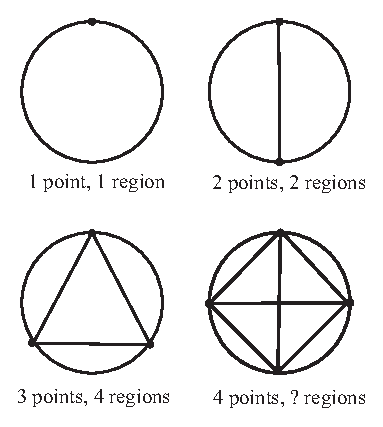
\includegraphics{figps-circleregions}
%%\caption{Regions of Circles} \label{fig:circleregions}
%\end{center}
%\end{figure}
%
%Count the number of distinct regions within each circle.  For example, with three points on the circle, there are four distinct regions.  Organize your data in a table with two columns: ``Number of Points on the Circle'' and ``Number of Distinct Regions in the Circle.''
%\begin{enumerate}
%\item Explain why there is only one region when there is one point on the circle and why there are two regions when there are two equally spaced points on the circle.  There are four regions when there are three equally spaced points on the circle.  How many regions are there when there are four equally spaced points on the circle?
%\item Based on the work so far, make a conjecture about how many distinct regions would you get with  five  equally spaced points and with six equally spaced points. \label{exer:circleregions1}
%
%%\item Based on the work so far, make a conjecture about how many distinct regions would you get with  six  equally spaced points. \label{exer:circleregions2}
%
%\item The following figure shows a circle with five equally space points and a circle with six equally spaced points.  Count the number of regions in each case.  Are your conjectures correct or incorrect?
%
%\begin{figure}[h]
%\begin{center}
%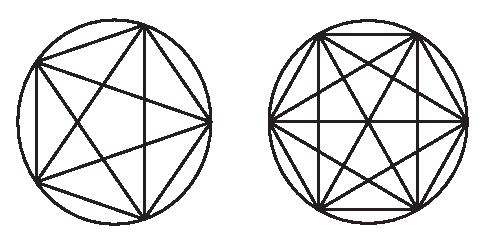
\includegraphics{figps-circle5-6.eps}
%%\caption{Regions of Circles} \label{fig:circleregions56}
%\end{center}
%\end{figure}
%
%\item What is the purpose of this exercise?
%\end{enumerate}

\item  \label{exer:derivatives} 
Let  $a$  be a real number.  We will explore the derivatives of the function 
$f\left( x \right) = e^{ax} $.  By using the chain rule, we see
\[
\frac{d}
{{dx}}\left( {e^{ax} } \right) = ae^{ax}. 
\]
Recall that the second derivative of a function is the derivative of the derivative function.  Similarly, the third derivative is the derivative of the second derivative.

\begin{enumerate}
\item What is  $\dfrac{{d^2 }}{{dx^2 }}\left( {e^{ax} } \right)$, the second derivative of   
$e^{ax} $?
	
\item What is  $\dfrac{{d^3 }}{{dx^3 }}\left( {e^{ax} } \right)$, the third derivative of   
$e^{ax} $?

\item Let  $n$  be a natural number.  Make a conjecture about the $n^{\text{th}}$ derivative of the function  $f\left( x \right) = e^{ax} $.  That is,  what is  
$\dfrac{{d^n }}{{dx^n }}\left( {e^{ax} } \right)$?  This conjecture should be written as a self-contained proposition including an appropriate quantifier.

\item Use mathematical induction to prove your conjecture.
\end{enumerate}
%\hbreak


\item In calculus, it can be shown that
\label{exer:wallis}%
\begin{align*}
\int_{}^{} \sin^{\,2} x \, dx &= \frac{x}{2} - \frac{1}{2} \sin x \cos x + c \quad \text{and} \\
\int_{}{} \cos^{\,2} x \, dx &= \frac{x}{2} + \frac{1}{2} \sin x \cos x + c.
\end{align*}
Using integration by parts, it is also possible to prove that for each natural number $n$,
\begin{align*}
\int_{}{} \sin^{\,n} x \, dx &= -\frac{1}{n} \sin^{n-1}x \cos x + \frac{n-1}{n} 
\int{}{} \sin^{\,n-2}x \, dx \quad \text{and} \\
\int_{}{} \cos^{\,n} x \, dx &= \frac{1}{n} \cos^{n-1}x \sin x + \frac{n-1}{n} 
\int{}{} \cos^{\,n-2}x \, dx.
\end{align*}

\begin{enumerate}
\item  Determine the values of 
\[
\int_{0}^{\pi/2} \sin^{\,2} x \, dx \qquad \text{and} \qquad 
\int_{0}^{\pi/2} \sin^{\,4} x \, dx.
\]
\item Use mathematical induction to prove that for each natural number $n$, 
\begin{align*}
\int_{0}^{\pi/2} \sin^{\,2n}x \, dx &= \frac{1 \cdot 3 \cdot 5 \cdots (2n - 1)}{2 \cdot 4 \cdot 6 \cdots (2n)} \frac{\pi}{2} \quad \text{and} \\
\int_{0}^{\pi/2} \sin^{\,2n+1}x \, dx &= \frac{2 \cdot 4 \cdot 6 \cdots (2n)}{1 \cdot 3  \cdot 5 \cdots (2n + 1)}. 
\end{align*}
These are known as the \textbf{\emph{Wallis sine formulas}}.
\index{Wallis sine formulas}%
%\item  Determine the values of 
%\[
%\int_{0}^{\pi/2} \cos^{\,2} x \, dx \qquad \text{and} \qquad 
%\int_{0}^{\pi/2} \cos^{\,4} x \, dx.
%\]
\item Use mathematical induction to prove that
\begin{align*}
\int_{0}^{\pi/2} \cos^{\,2n}x \, dx &= \frac{1 \cdot 3 \cdot 5 \cdots (2n - 1)}{2 \cdot 4 \cdot 6 \cdots (2n)} \frac{\pi}{2} \quad \text{and} \\
\int_{0}^{\pi/2} \cos^{\,2n+1}x \, dx &= \frac{2 \cdot 4 \cdot 6 \cdots (2n)}{1 \cdot 3 \cdot 5 \cdots (2n+1)}.
\end{align*}
These are known as the \textbf{\emph{Wallis cosine formulas}}.
\index{Wallis cosine formulas}%
\end{enumerate}


\item \begin{enumerate}
\item Why is it not possible to use mathematical induction to prove a proposition of the form
\[
\left( {\forall x \in \mathbb{Q}} \right)\left( {P( x )} \right),
\]
where  $P( x )$ is some predicate?

\item Why is it not possible to use mathematical induction to prove a proposition of the form
\begin{center}
For each real number  $x$  with  $x \geq 1$,  $P( x )$,
\end{center}
where  $P( x )$ is some predicate?
\end{enumerate}

\item \textbf{Evaluation of proofs}  \hfill \\
See the instructions for Exercise~(\ref{exer:proofeval}) on 
page~\pageref{exer:proofeval} from Section~\ref{S:directproof}.

\begin{enumerate}
\item For each natural number $n$, $1 + 4 + 7 + \cdots + \left( 3n - 2 \right) = 
\dfrac{n \left(3n - 1 \right)}{2}$.

\begin{myproof}
We will prove this proposition using mathematical induction.  So we let $P ( n )$ be the open sentence
\[
1 + 4 + 7 + \cdots + \left( 3n - 2 \right)\!.
\]
Using $n = 1$, we see that $3n - 2 = 1$ and hence, $P \left( 1 \right)$ is true.

We now assume that $P( k )$ is true.  That is, 
\[
1 + 4 + 7 + \cdots + \left( 3k - 2 \right) = \frac{k \left(3k -1 \right)}{2} .
\]
We then see that
\[
\begin{aligned}
1 + 4 + 7 + \cdots + \left( 3k - 2 \right) + \left( 3 (k + 1) - 2 \right) &= 
    \frac{\left(k + 1 \right) \left(3k + 2 \right)}{2} \\
\frac{k \left(3k -1 \right)}{2} + \left(3k + 1 \right) &= \frac{\left(k + 1 \right) \left(3k + 2 \right)}{2} \\
\frac{\left(3k^2 - k \right) + \left(6k + 2 \right) }{2} &= \frac{3k^2 + 5k + 2}{2} \\
\frac{3k^2 +5k + 2}{2} &=  \frac{3k^2 + 5k + 2}{2}.        
\end{aligned}
\]

We have thus proved that $P( k + 1 )$ is true, and hence, we have proved the proposition.
\end{myproof}


\item For each natural number $n$, $1 + 4 + 7 + \cdots + \left( 3n - 2 \right) = 
\dfrac{n \left(3n - 1 \right)}{2}$.

\begin{myproof}
We will prove this proposition using mathematical induction.  So we let

\[
P( n ) = 1 + 4 + 7 + \cdots + \left( 3n - 2 \right)\!.
\]

Using $n = 1$, we see that $P( 1 ) = 1$ and hence, $P( 1 )$ is true.

We now assume that $P( k )$ is true.  That is, 

\[
1 + 4 + 7 + \cdots + \left( 3k - 2 \right) = \frac{k \left(3k -1 \right)}{2} .
\]

We then see that

\[
\begin{aligned}
P( k + 1 ) &= 1 + 4 + 7 + \cdots + \left( 3k - 2 \right) + \left( 3 (k + 1) - 2 \right) \\
                       &= \frac{k \left( 3k - 1 \right)}{2} + 3 \left(k + 1 \right) - 2 \\
                       &= \frac{3k^2 - k + 6k + 6 - 4}{2} \\
                       &= \frac{3k^2 + 5k + 2}{2} \\
                       &= \frac{\left(k + 1 \right) \left(3k + 2 \right)}{2}.
\end{aligned}
\]

We have thus proved that $P( k + 1 )$ is true, and hence, we have proved the proposition.
\end{myproof}
%\item For each natural number $n$, $1 + 3 + 5 + \cdots + \left( 2n - 1 \right) = n^2$.
%
%\begin{myproof}
%We will prove this proposition using mathematical induction.  So we let
%
%\[
%P \left( n \right) = 1 + 3 + 5 + \cdots + \left( 2n - 1 \right).
%\]
%
%Using $n = 1$, we see that $P \left( 1 \right) = 1$ and hence, $P \left( 1 \right)$ is true.
%
%We now assume that $P \left( k \right)$ is true.  That is, 
%
%\[
%1 + 3 + 5 + \cdots + \left( 2k - 1 \right) = k^2.
%\]
%
%We then see that
%
%\[
%\begin{aligned}
%P \left( k + 1 \right) &= 1 + 3 + 5 + \cdots + \left( 2k - 1 \right) + \left( 2 (k + 1) - 1 \right) \\
%                       &= k^2 + 2k + 1 \\
%                       &= \left( k + 1 \right)^2.
%\end{aligned}
%\]
%
%We have thus proved that $P \left( k + 1 \right)$ is true, and hence, we have proved the proposition.
%\end{myproof}

\item All dogs are the same breed.

\begin{myproof}
We will prove this proposition using mathematical induction.  For each natural number $n$, we let 
$P( n )$ be

\begin{center}
Any set of $n$ dogs consists entirely of dogs of the same breed.
\end{center}

We will prove that for each natural number $n$, $P( n )$ is true, which will prove that all dogs are the same breed.  A set with only one dog consists entirely of dogs of the same breed and,  hence, $P( 1 )$ is true.

So we let $k$ be a natural number and assume that $P( k )$ is true, that is, that every set of 
$k$ dogs consists of dogs of the same breed.  Now consider a set $D$ of $k + 1$ dogs, where

\[
D = \left\{ d_1, d_2, \ldots, d_k, d_{k+1} \right\}\!.
\]

If we remove the dog $d_1$ from the set $D$, we then have a set $D_1$ of $k$ dogs, and using the assumption that $P( k )$ is true, these dogs must all be of the same breed.  Similarly, if we remove $d_{k+1}$ from the set $D$, we again have a set $D_2$ of $k$ dogs, and these dogs must all be of the same breed.  Since $D = D_1 \cup D_2$, we have proved that all of the dogs in $D$ must be of the same breed.

This proves that if $P( k )$ is true, then $P( k + 1 )$ is true and, hence, by mathematical induction, we have proved that for each natural number $n$, any set of $n$ dogs consists entirely of dogs of the same breed.
\end{myproof}
\end{enumerate}
\end{enumerate}


\subsection*{Explorations and Activities}
\setcounter{oldenumi}{\theenumi}
\begin{enumerate} \setcounter{enumi}{\theoldenumi} \setcounter{equation}{0}
  \item \textbf{The Importance of the Basis Step}.  \label{exer:basis} Most of the work done in constructing a proof by induction is usually in proving the inductive step.  This was certainly the case in Proposition~\ref{P:suminduction}.  However, the basis step is an essential part of the proof. Without it, the proof is incomplete.  To see this, let 
$P( n )$   be 
\[
1 + 2 +  \cdots  + n = \frac{{n^2  + n + 1}}{2}.
\]
\begin{enumerate}
  \item Let  $k \in \mathbb{N}$.  Complete the following proof that if  $P(  k )$ is true, then  $P( k + 1 )$ is true.

Let  $k \in \mathbb{N}$.  Assume that  $P(  k )$ is true.  That is, assume that
%
\begin{equation} \label{eq:act16a}
1 + 2 +  \cdots  + k = \frac{{k^2  + k + 1}}{2}.
\end{equation}
%
The goal is to prove that  $P( k + 1 )$ is true.  That is, we need to prove that
%
\begin{equation} \label{eq:act16b}
1 + 2 +  \cdots  + k + \left( {k + 1} \right) = \frac{{\left( {k + 1} \right)^2  + \left( {k + 1} \right) + 1}}{2}.
\end{equation}
%
To do this, we add  $\left( {k + 1} \right)$ to both sides of equation~(\ref{eq:act16a}).  This gives
\[
\begin{aligned}
  1 + 2 +  \cdots  + k + \left( {k + 1} \right) &= \frac{{k^2  + k + 1}}{2} + \left( {k + 1} \right) \\ 
                                                &=  \cdots.  \\ 
\end{aligned}
\]

  \item Is  $P( 1 )$ true?  Is  $P( 2 )$ true?  What about $P( 3 )$ and $P( 4 )$?  Explain how this shows that the basis step is an essential part of a proof by induction.
\end{enumerate}

\item \textbf{Regions of a Circle}. \label{exer:circleregions} Place  $n$  equally spaced points on a circle and connect each pair of points with the chord of the circle determined by that pair of points.  See Figure~\ref{fig:circleregions}.

\begin{figure}[h]
\begin{center}
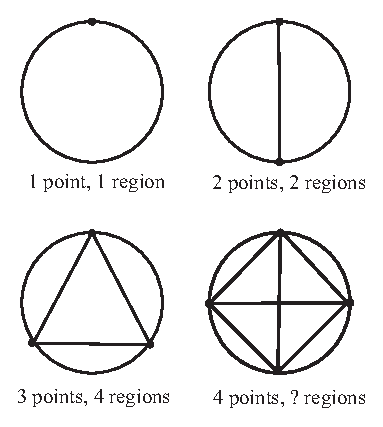
\includegraphics{figps-circleregions}
\caption{Regions of Circles} \label{fig:circleregions}
\end{center}
\end{figure}
Count the number of distinct regions within each circle.  For example, with three points on the circle, there are four distinct regions.  Organize your data in a table with two columns: ``Number of Points on the Circle'' and ``Number of Distinct Regions in the Circle.''
\begin{enumerate}
\item How many regions are there when there are four equally spaced points on the circle?
\item Based on the work so far, make a conjecture about how many distinct regions would you get with  five  equally spaced points. \label{A:circleregions1}

\item Based on the work so far, make a conjecture about how many distinct regions would you get with  six  equally spaced points. \label{A:circleregions2}

\item Figure~\ref{fig:circleregions56} shows the figures associated with Parts~(b) and~(c).  Count the number of regions in each case.  Are your conjectures correct or incorrect?

\begin{figure}[h!]
\begin{center}
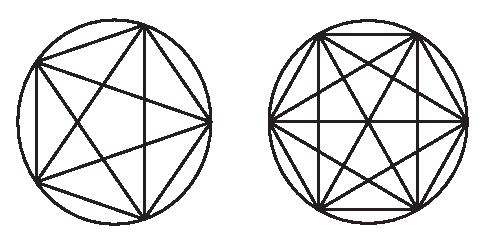
\includegraphics{figps-circle5-6.eps}
\caption{Regions of Circles} \label{fig:circleregions56}
\end{center}
\end{figure}

\item Explain why this activity shows that the inductive step is an essential part of a proof by mathematical induction.
\end{enumerate}

\end{enumerate}

\hbreak



\endinput

\item \begin{enumerate} \item In Section~\ref{S:provingset}, we learned how to use the \textbf{Choose Method}
\index{Choose Method}%
 to prove propositions of the form,
\begin{list}{}
  \item For all ``objects'' with a ``certain property'', ``something happens.''
\end{list}
Under what conditions would we consider using mathematical induction to prove such a proposition rather than the Choose Method?

